\documentclass[10pt]{beamer}

\usetheme{metropolis}
\usepackage{appendixnumberbeamer}
\usepackage{empheq}
\usepackage{pdfpages}
\usepackage{booktabs}
\usepackage{adjustbox}
\usepackage[scale=2]{ccicons}
\usepackage{tikz}
\usepackage{media9}

\usepackage{listings}


\usetikzlibrary{calc,shapes.callouts,shapes.arrows}
\newcommand{\deriv}{\stackrel{\leftrightarrow}{\partial}}
\newcommand{\derleft}{\stackrel{\leftarrow}{\partial}}
\newcommand{\derright}{\stackrel{\rightarrow}{\partial}}
\newcommand{\vect}[1]{\boldsymbol{\rm #1}}
\newcommand{\ev}[1]{\ensuremath{\left\langle #1 \right\rangle}} %
\newcommand{\Ho}{H_{1\textrm{DM}}}
\newcommand{\Ht}{H_{2\textrm{DM}}}
\renewcommand{\L}{\mathcal{L}}
\newcommand{\D}{\mathcal{D}}
\newcommand{\T}{\mathcal{T}}
\newcommand{\speechthis}[2]{
	\tikz[remember picture,baseline]{\node[anchor=base,inner sep=0,outer sep=0]%
		(#1) {\underline{#1}};\node[overlay,ellipse callout,fill=blue!50] 
		at ($(#1.north)+(-.5cm,0.8cm)$) {#2};}%
}%
% Maths Packages
\usepackage{amsmath}
\usepackage{amsfonts}
\usepackage{amssymb}
%\usepackage{physics}
\usepackage{slashed}

% Graphics Packages
\usepackage{graphicx}
\usepackage{float}
\usepackage{xcolor}
\usepackage{caption}
\usepackage{subcaption}


%\fontfamily{qag}\selectfont

%\useoutertheme{infolines}
%\useinnertheme{rounded}

%% Changeing the font
\setbeamerfont{caption}{size=\scriptsize}
\setbeamertemplate{caption}[numbered]
%\usepackage[default]{charter}
%\usepackage{fontenc}
%\usefont{}

% Defining colours
\definecolor{cream}{RGB}{253,255,255}
\definecolor{dGreen}{RGB}{20,50,50}
\definecolor{lGreen}{RGB}{242,250,250}
\definecolor{white}{RGB}{255,255,255}
\definecolor{orange}{RGB}{230,140,50}
\definecolor{lPurple}{RGB}{250,240,255}
\definecolor{dPurple}{RGB}{40,20,50}

% Setting colours
\setbeamercolor{background canvas}{bg=white}

% Font Colours
\setbeamercolor{title}{fg=dGreen}
\setbeamercolor{normal text}{fg=dGreen,bg=white}
\setbeamercolor{frametitle}{fg=white,bg=dGreen=20}

\setbeamercolor{bibliography entry author}{fg=dGreen,bg=white}
\setbeamercolor{bibliography entry title}{fg=dGreen,bg=white} 
\setbeamercolor{bibliography entry location}{fg=dGreen,bg=white} 
\setbeamercolor{bibliography entry note}{fg=dGreen,bg=white}  

% Fixing lists
\setbeamertemplate{itemize items}[default]
\setbeamertemplate{enumerate items}[default]
\setbeamercolor{itemize item}{fg=orange}
\setbeamercolor{itemize subitem}{fg=orange}
\setbeamercolor{itemize subsubitem}{fg=orange}
\setbeamercolor{enumerate item}{fg=orange}
\setbeamercolor{enumerate subitem}{fg=orange}
\setbeamercolor{enumerate subsubitem}{fg=orange}

% Setting transperancy of unrevealed points
\setbeamercovered{transparent=20}

% Setting block parameters
\setbeamertemplate{blocks}[default]
\setbeamercolor{block title}{bg=dGreen,fg=white}
\setbeamercolor{block body}{bg=lGreen}

% Setting footnote parameters
\setbeamertemplate{footline}{{
          \makebox[\textwidth]{\hfill\makebox[20pt]{\color{dGreen}
          \scriptsize \insertframenumber / \inserttotalframenumber}}}\hspace*{5pt}}

%International Nuclear Physics Conference September 11-16, 2016

% Correcting bibliography style
\setbeamertemplate{bibliography item}{\insertbiblabel}

% Removing navigation symbols from bottom right.
\beamertemplatenavigationsymbolsempty


\usepackage{pgfplots}
\usepgfplotslibrary{dateplot}



\graphicspath{ {/home/andre/Uni/Dropbox/Project/Directional/tex_multi/v_2/figures/} {/home/andre/Uni/Dropbox/Project/Directional/tex_multi/v_2/paramEst/} }


\usepackage{xspace}
\newcommand{\themename}{\textbf{\textsc{metropolis}}\xspace}

\title{Getting an academic job (online).  }
\date{\today}
\author{Andre Scaffidi and Theo Motta }

%\titlegraphic{\hfill\includegraphics[height=1.0cm]{picture}}
%\titlegraphic{\hfill\includegraphics[height=1.0cm]{CoEPPlogo1}}


\begin{document}

\maketitle

\begin{frame}{Contents}
\tableofcontents
\end{frame}


\section{How to apply for a postdoctoral job: The websites you need to know}

\begin{frame}{Academic jobs online}
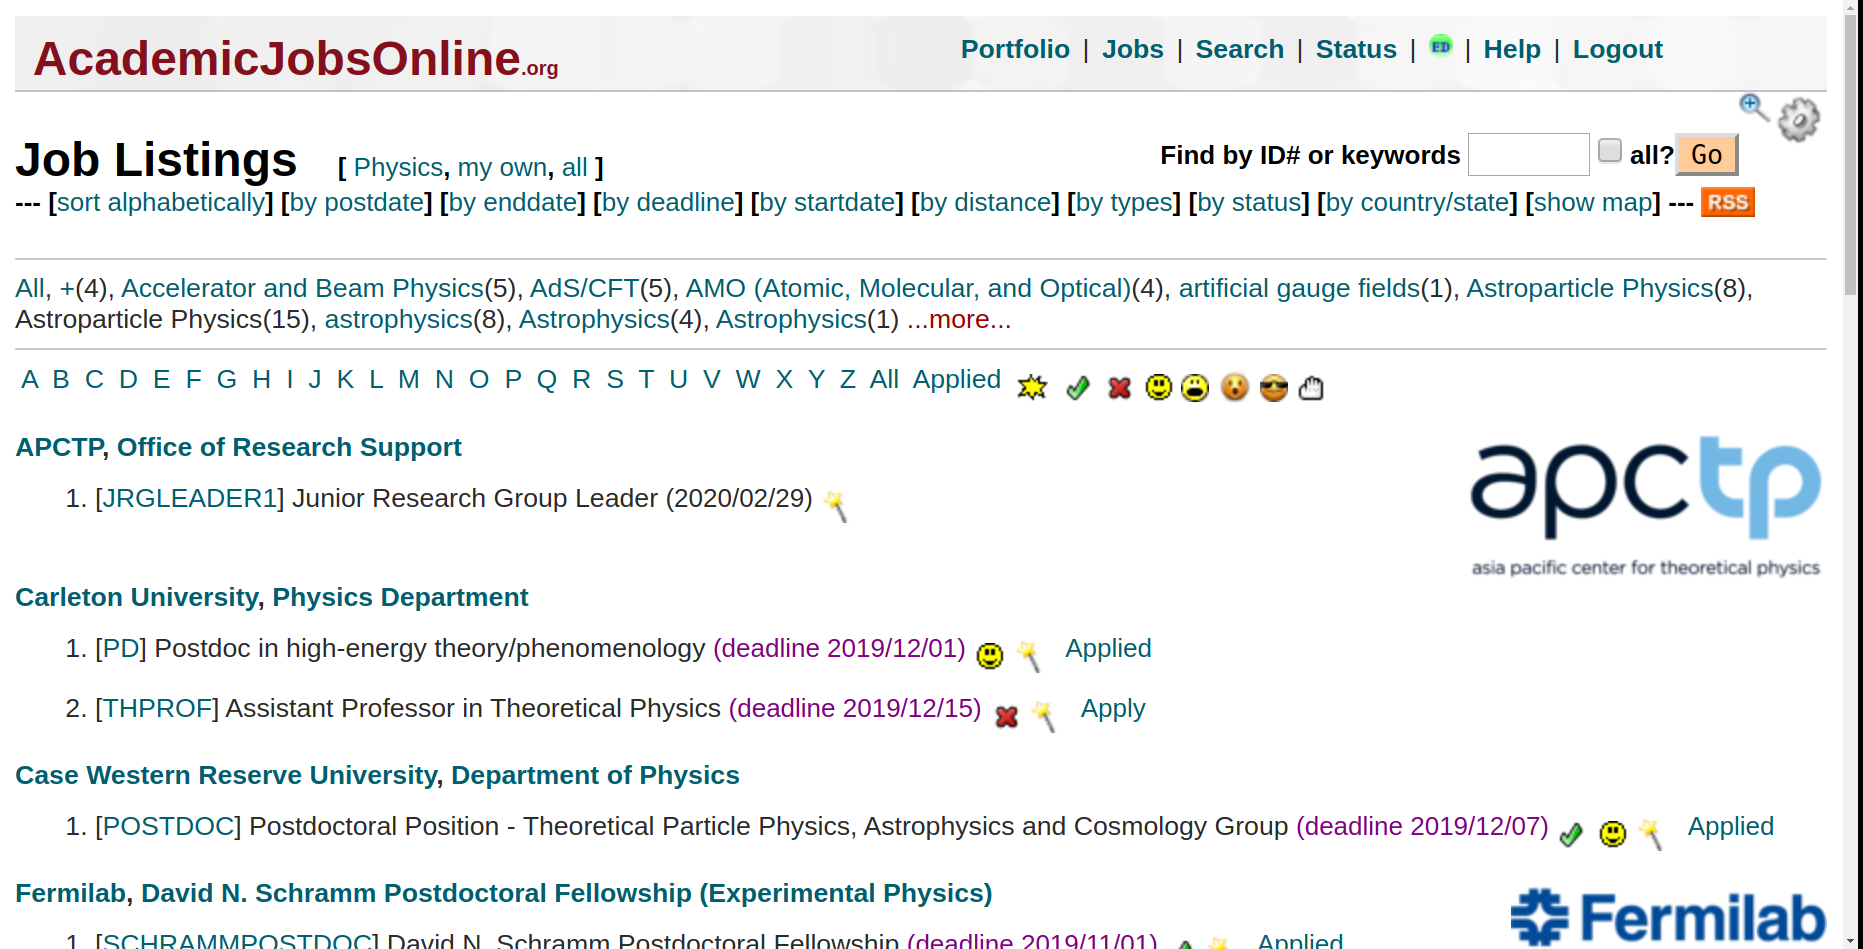
\includegraphics[width=\textwidth]{ajo}
\begin{itemize}
	\item US, Asia/Oceania and most* Europe jobs. 
	\item Referees upload letters ONCE. AJO will send letters to employer. 
	\item Can upload DEFAULT CV/research statement/cover letter. 
\end{itemize}
\end{frame}
\begin{frame}{Inspire Jobs}
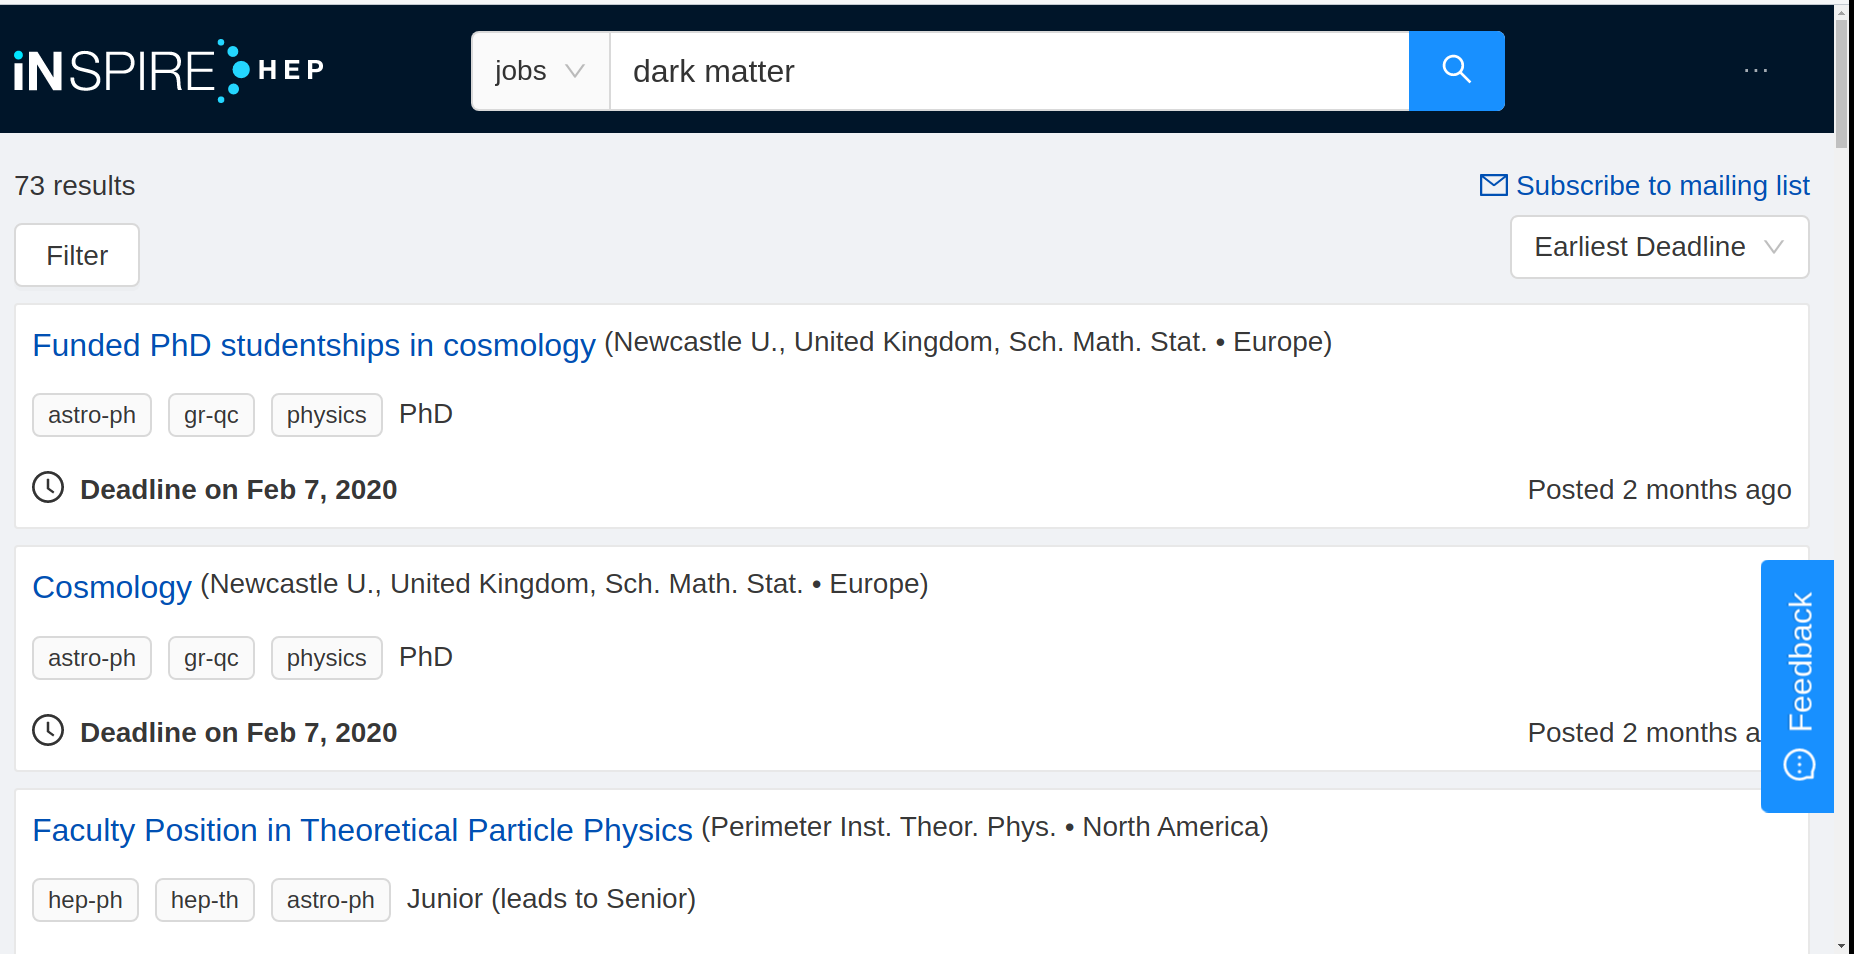
\includegraphics[width=\textwidth]{inspire_job}
\begin{itemize}
	\item Most jobs posted here. However this round AJO did really well...
	\item Need to email reference letters individually $<$--- Sucks!
\end{itemize}
\end{frame}

\section{The cover letter, research statement and CV}
\begin{frame}
Ideas to talk about
\begin{itemize}
	\item Length of each
	\item their names not sir/madam
	\item research statement most important!?
	\item Can get interview based off statement. 
\end{itemize}

\end{frame}
\section{The ``main round": Structure and important dates}
\begin{frame}
Ideas to talk about
	\begin{itemize}
		\item Define main round (for hep only really?)
		\item Andre: Experience off main round with slovenia 
		\item Jan 7th!!!!!
		\item best people get poached first. This year CERN got 5 people in November
	\end{itemize}

\end{frame}


\section{Rumour mill}
\begin{frame}
\begin{itemize}
	\item overview of what it is
		\item (maybe?) scrape rumor mill stats for job offers
		\item rumour mill psychology
		\item shit people get the offers  - who they know 
		\item 
\end{itemize}
\end{frame}


\section{The interview}
\begin{frame}
Ideas to talk about
\begin{itemize}
	\item NOT like industry
	\item Very very chilled.
	\item IF they talk about anything, it will only be about research statement. 
	\item know what job you are applying for lol
\end{itemize}

\end{frame}

\end{document}
